\subsection{Photovoltaic energy yield} \label{sec:energy_yield}
As already mentioned in subsection \ref{sec:solar_irradiation_on_earths_surface} the decisive factors to determine the irradiance at a given location on the Earth's surface are the GHI and the DNI. Building on these, the three-component model as described in \cite{Landis:1995, Mertens:2015}, can be used to calculate the \emph{total irradiance} $E_{\mathrm{G}}$ in $\left( \mathrm{W}\mathrm{m}^{-2} \right)$ received by an inclined PV generator. The \emph{angle of inclination} with respect to the ground is $\beta$ in $\left( ^\circ \right)$. An example for such an inclined PV generator can be seen in the figures \ref{fig:tikz_three_component_model} and \ref{fig:tikz_angle_theta}.
\begin{figure}[h!]
	\centering
	

\tikzset{every picture/.style={line width=0.75pt}} %set default line width to 0.75pt        

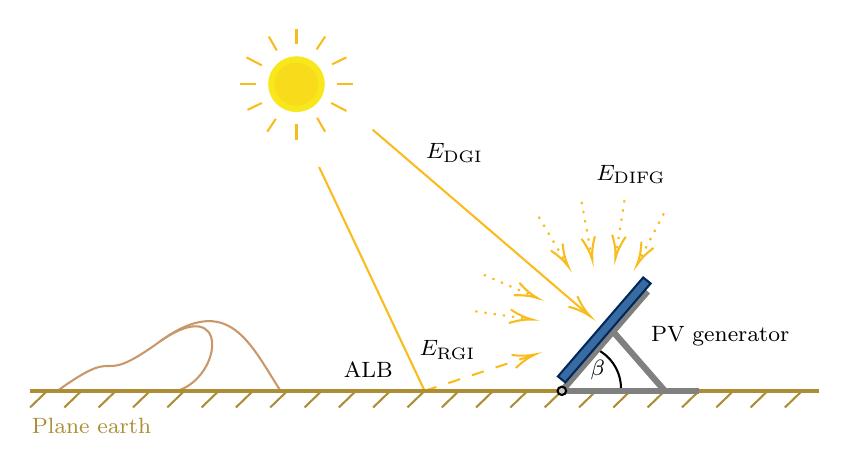
\begin{tikzpicture}[x=0.75pt,y=0.75pt,yscale=-1,xscale=1]
%uncomment if require: \path (0,468); %set diagram left start at 0, and has height of 468

%Straight Lines [id:da7639591375517361] 
\draw [color={rgb, 255:red, 248; green, 189; blue, 28 }  ,draw opacity=1 ]   (249.06,186.64) -- (299.9,294.48) ;
%Shape: Ellipse [id:dp07145193932966887] 
\draw  [color={rgb, 255:red, 248; green, 231; blue, 28 }  ,draw opacity=1 ][fill={rgb, 255:red, 248; green, 220; blue, 28 }  ,fill opacity=1 ][line width=2.25]  (226.02,146.71) .. controls (226.02,140.12) and (231.45,134.77) .. (238.15,134.77) .. controls (244.85,134.77) and (250.29,140.12) .. (250.29,146.71) .. controls (250.29,153.31) and (244.85,158.65) .. (238.15,158.65) .. controls (231.45,158.65) and (226.02,153.31) .. (226.02,146.71) -- cycle ;
%Curve Lines [id:da4839167804983171] 
\draw [color={rgb, 255:red, 202; green, 151; blue, 106 }  ,draw opacity=1 ]   (172.61,270.51) .. controls (206.08,247.35) and (202.78,287.29) .. (180.87,294.48) ;
%Curve Lines [id:da9367845814708875] 
\draw [color={rgb, 255:red, 202; green, 151; blue, 106 }  ,draw opacity=1 ]   (123.01,294.48) .. controls (156.08,270.51) and (139.55,294.48) .. (172.61,270.51) .. controls (205.67,246.55) and (216,272.11) .. (230.47,294.48) ;
%Straight Lines [id:da20208524763476388] 
\draw [color={rgb, 255:red, 248; green, 189; blue, 28 }  ,draw opacity=1 ] [dash pattern={on 4.5pt off 4.5pt}]  (299.9,294.48) -- (351.31,277.53) ;
\draw [shift={(353.21,276.9)}, rotate = 521.76] [color={rgb, 255:red, 248; green, 189; blue, 28 }  ,draw opacity=1 ][line width=0.75]    (10.93,-3.29) .. controls (6.95,-1.4) and (3.31,-0.3) .. (0,0) .. controls (3.31,0.3) and (6.95,1.4) .. (10.93,3.29)   ;
%Curve Lines [id:da8387867434601526] 
\draw    (382.96,274.51) .. controls (387.92,276.9) and (394.53,283.29) .. (394.53,293.68) ;
%Straight Lines [id:da056555134551903974] 
\draw [color={rgb, 255:red, 173; green, 142; blue, 55 }  ,draw opacity=1 ][fill={rgb, 255:red, 139; green, 87; blue, 42 }  ,fill opacity=1 ][line width=1.5]    (109.79,294.48) -- (490,294.48) ;
%Straight Lines [id:da48348316265398994] 
\draw [color={rgb, 255:red, 173; green, 142; blue, 55 }  ,draw opacity=1 ]   (134.59,294.48) -- (126.32,302.47) ;
%Straight Lines [id:da4565238298434817] 
\draw [color={rgb, 255:red, 173; green, 142; blue, 55 }  ,draw opacity=1 ]   (151.12,294.48) -- (142.85,302.47) ;
%Straight Lines [id:da7555358341240341] 
\draw [color={rgb, 255:red, 173; green, 142; blue, 55 }  ,draw opacity=1 ]   (167.65,294.48) -- (159.38,302.47) ;
%Straight Lines [id:da10247707612378121] 
\draw [color={rgb, 255:red, 173; green, 142; blue, 55 }  ,draw opacity=1 ]   (184.18,294.48) -- (175.91,302.47) ;
%Straight Lines [id:da22505664528789526] 
\draw [color={rgb, 255:red, 173; green, 142; blue, 55 }  ,draw opacity=1 ]   (200.71,294.48) -- (192.44,302.47) ;
%Straight Lines [id:da39883233893640213] 
\draw [color={rgb, 255:red, 173; green, 142; blue, 55 }  ,draw opacity=1 ]   (217.24,294.48) -- (208.98,302.47) ;
%Straight Lines [id:da9317267044471207] 
\draw [color={rgb, 255:red, 173; green, 142; blue, 55 }  ,draw opacity=1 ]   (233.77,294.48) -- (225.51,302.47) ;
%Straight Lines [id:da5689034971431022] 
\draw [color={rgb, 255:red, 173; green, 142; blue, 55 }  ,draw opacity=1 ]   (118.06,294.48) -- (109.79,302.47) ;
%Straight Lines [id:da6794614658982192] 
\draw [color={rgb, 255:red, 173; green, 142; blue, 55 }  ,draw opacity=1 ]   (250.3,294.48) -- (242.04,302.47) ;
%Straight Lines [id:da16884333894084147] 
\draw [color={rgb, 255:red, 173; green, 142; blue, 55 }  ,draw opacity=1 ]   (266.83,294.48) -- (258.57,302.47) ;
%Straight Lines [id:da5852948402158396] 
\draw [color={rgb, 255:red, 173; green, 142; blue, 55 }  ,draw opacity=1 ]   (283.36,294.48) -- (275.1,302.47) ;
%Straight Lines [id:da5569944189270981] 
\draw [color={rgb, 255:red, 173; green, 142; blue, 55 }  ,draw opacity=1 ]   (299.9,294.48) -- (291.63,302.47) ;
%Straight Lines [id:da07636127130608306] 
\draw [color={rgb, 255:red, 173; green, 142; blue, 55 }  ,draw opacity=1 ]   (316.43,294.48) -- (308.16,302.47) ;
%Straight Lines [id:da7270434905185723] 
\draw [color={rgb, 255:red, 173; green, 142; blue, 55 }  ,draw opacity=1 ]   (332.96,294.48) -- (324.69,302.47) ;
%Straight Lines [id:da5998901663023846] 
\draw [color={rgb, 255:red, 173; green, 142; blue, 55 }  ,draw opacity=1 ]   (349.49,294.48) -- (341.22,302.47) ;
%Straight Lines [id:da2586618910795322] 
\draw [color={rgb, 255:red, 173; green, 142; blue, 55 }  ,draw opacity=1 ]   (366.02,294.48) -- (357.75,302.47) ;
%Straight Lines [id:da2230405823513728] 
\draw [color={rgb, 255:red, 173; green, 142; blue, 55 }  ,draw opacity=1 ]   (382.55,294.48) -- (374.28,302.47) ;
%Straight Lines [id:da33268357962040995] 
\draw [color={rgb, 255:red, 173; green, 142; blue, 55 }  ,draw opacity=1 ]   (399.08,294.48) -- (390.81,302.47) ;
%Straight Lines [id:da9040529515577587] 
\draw [color={rgb, 255:red, 173; green, 142; blue, 55 }  ,draw opacity=1 ]   (415.61,294.48) -- (407.35,302.47) ;
%Straight Lines [id:da9864302443455792] 
\draw [color={rgb, 255:red, 173; green, 142; blue, 55 }  ,draw opacity=1 ]   (432.14,294.48) -- (423.88,302.47) ;
%Straight Lines [id:da5062470043832821] 
\draw [color={rgb, 255:red, 173; green, 142; blue, 55 }  ,draw opacity=1 ]   (448.67,294.48) -- (440.41,302.47) ;
%Straight Lines [id:da3838353864046502] 
\draw [color={rgb, 255:red, 173; green, 142; blue, 55 }  ,draw opacity=1 ]   (465.2,294.48) -- (456.94,302.47) ;
%Straight Lines [id:da7629428788396968] 
\draw [color={rgb, 255:red, 173; green, 142; blue, 55 }  ,draw opacity=1 ]   (481.73,294.48) -- (473.47,302.47) ;
%Straight Lines [id:da014514371361068923] 
\draw [color={rgb, 255:red, 128; green, 128; blue, 128 }  ,draw opacity=1 ][line width=2.25]    (407.35,246.55) -- (366.02,294.48) ;
%Straight Lines [id:da49954840219882635] 
\draw [color={rgb, 255:red, 128; green, 128; blue, 128 }  ,draw opacity=1 ][line width=2.25]    (432.14,294.48) -- (366.02,294.48) ;
%Straight Lines [id:da9965546684463125] 
\draw [color={rgb, 255:red, 128; green, 128; blue, 128 }  ,draw opacity=1 ][line width=2.25]    (391.23,266.52) -- (415.61,294.48) ;
%Straight Lines [id:da9786945806038319] 
\draw [color={rgb, 255:red, 248; green, 189; blue, 28 }  ,draw opacity=1 ] [dash pattern={on 0.84pt off 2.51pt}]  (415.2,209.01) -- (403.11,232) ;
\draw [shift={(402.18,233.77)}, rotate = 297.73] [color={rgb, 255:red, 248; green, 189; blue, 28 }  ,draw opacity=1 ][line width=0.75]    (10.93,-3.29) .. controls (6.95,-1.4) and (3.31,-0.3) .. (0,0) .. controls (3.31,0.3) and (6.95,1.4) .. (10.93,3.29)   ;
%Straight Lines [id:da4673310913126938] 
\draw [color={rgb, 255:red, 248; green, 189; blue, 28 }  ,draw opacity=1 ] [dash pattern={on 0.84pt off 2.51pt}]  (324.28,256.14) -- (349.78,259.84) ;
\draw [shift={(351.76,260.13)}, rotate = 188.27] [color={rgb, 255:red, 248; green, 189; blue, 28 }  ,draw opacity=1 ][line width=0.75]    (10.93,-3.29) .. controls (6.95,-1.4) and (3.31,-0.3) .. (0,0) .. controls (3.31,0.3) and (6.95,1.4) .. (10.93,3.29)   ;
%Straight Lines [id:da559627746158232] 
\draw [color={rgb, 255:red, 248; green, 189; blue, 28 }  ,draw opacity=1 ] [dash pattern={on 0.84pt off 2.51pt}]  (328.41,238.56) -- (352.4,248.95) ;
\draw [shift={(354.24,249.75)}, rotate = 203.41] [color={rgb, 255:red, 248; green, 189; blue, 28 }  ,draw opacity=1 ][line width=0.75]    (10.93,-3.29) .. controls (6.95,-1.4) and (3.31,-0.3) .. (0,0) .. controls (3.31,0.3) and (6.95,1.4) .. (10.93,3.29)   ;
%Straight Lines [id:da4533498063566359] 
\draw [color={rgb, 255:red, 248; green, 189; blue, 28 }  ,draw opacity=1 ] [dash pattern={on 0.84pt off 2.51pt}]  (375.52,203.42) -- (380.33,229.41) ;
\draw [shift={(380.69,231.37)}, rotate = 259.53] [color={rgb, 255:red, 248; green, 189; blue, 28 }  ,draw opacity=1 ][line width=0.75]    (10.93,-3.29) .. controls (6.95,-1.4) and (3.31,-0.3) .. (0,0) .. controls (3.31,0.3) and (6.95,1.4) .. (10.93,3.29)   ;
%Straight Lines [id:da995866694125163] 
\draw [color={rgb, 255:red, 248; green, 189; blue, 28 }  ,draw opacity=1 ] [dash pattern={on 0.84pt off 2.51pt}]  (396.19,202.62) -- (392.15,228.6) ;
\draw [shift={(391.85,230.57)}, rotate = 278.82] [color={rgb, 255:red, 248; green, 189; blue, 28 }  ,draw opacity=1 ][line width=0.75]    (10.93,-3.29) .. controls (6.95,-1.4) and (3.31,-0.3) .. (0,0) .. controls (3.31,0.3) and (6.95,1.4) .. (10.93,3.29)   ;
%Straight Lines [id:da13557132527331994] 
\draw [color={rgb, 255:red, 248; green, 189; blue, 28 }  ,draw opacity=1 ] [dash pattern={on 0.84pt off 2.51pt}]  (354.86,210.6) -- (368.1,232.85) ;
\draw [shift={(369.12,234.57)}, rotate = 239.25] [color={rgb, 255:red, 248; green, 189; blue, 28 }  ,draw opacity=1 ][line width=0.75]    (10.93,-3.29) .. controls (6.95,-1.4) and (3.31,-0.3) .. (0,0) .. controls (3.31,0.3) and (6.95,1.4) .. (10.93,3.29)   ;
%Shape: Ellipse [id:dp027496909576239847] 
\draw  [fill={rgb, 255:red, 202; green, 202; blue, 202 }  ,fill opacity=1 ] (363.95,294.48) .. controls (363.95,293.37) and (364.88,292.48) .. (366.02,292.48) .. controls (367.16,292.48) and (368.08,293.37) .. (368.08,294.48) .. controls (368.08,295.58) and (367.16,296.47) .. (366.02,296.47) .. controls (364.88,296.47) and (363.95,295.58) .. (363.95,294.48) -- cycle ;
%Straight Lines [id:da8059435922738829] 
\draw [color={rgb, 255:red, 248; green, 189; blue, 28 }  ,draw opacity=1 ]   (274.89,168.67) -- (378.14,257.23) ;
\draw [shift={(379.66,258.53)}, rotate = 220.62] [color={rgb, 255:red, 248; green, 189; blue, 28 }  ,draw opacity=1 ][line width=0.75]    (10.93,-3.29) .. controls (6.95,-1.4) and (3.31,-0.3) .. (0,0) .. controls (3.31,0.3) and (6.95,1.4) .. (10.93,3.29)   ;
%Straight Lines [id:da20746203736647328] 
\draw [color={rgb, 255:red, 248; green, 189; blue, 28 }  ,draw opacity=1 ]   (238.15,120) -- (238.15,127.43) ;
%Straight Lines [id:da7474001161810504] 
\draw [color={rgb, 255:red, 248; green, 189; blue, 28 }  ,draw opacity=1 ]   (265.3,146.71) -- (257.75,146.71) ;
%Straight Lines [id:da2676635751494898] 
\draw [color={rgb, 255:red, 248; green, 189; blue, 28 }  ,draw opacity=1 ]   (238.15,173.43) -- (238.15,165.99) ;
%Straight Lines [id:da5591085501687709] 
\draw [color={rgb, 255:red, 248; green, 189; blue, 28 }  ,draw opacity=1 ]   (218.55,146.71) -- (211,146.71) ;
%Straight Lines [id:da29943329422514986] 
\draw [color={rgb, 255:red, 248; green, 189; blue, 28 }  ,draw opacity=1 ]   (254.9,155.79) -- (262.18,159.61) ;
%Straight Lines [id:da8331061745611166] 
\draw [color={rgb, 255:red, 248; green, 189; blue, 28 }  ,draw opacity=1 ]   (214.12,133.82) -- (221.41,137.64) ;
%Straight Lines [id:da7334533162645056] 
\draw [color={rgb, 255:red, 248; green, 189; blue, 28 }  ,draw opacity=1 ]   (262.18,133.82) -- (255.32,137.16) ;
%Straight Lines [id:da16844895743023902] 
\draw [color={rgb, 255:red, 248; green, 189; blue, 28 }  ,draw opacity=1 ]   (221.41,155.79) -- (214.55,159.13) ;
%Straight Lines [id:da941363141001635] 
\draw [color={rgb, 255:red, 248; green, 189; blue, 28 }  ,draw opacity=1 ]   (247.86,129.97) -- (251.98,123.79) ;
%Straight Lines [id:da8944108780017783] 
\draw [color={rgb, 255:red, 248; green, 189; blue, 28 }  ,draw opacity=1 ]   (224.07,169.61) -- (228.2,163.43) ;
%Straight Lines [id:da6072002125224827] 
\draw [color={rgb, 255:red, 248; green, 189; blue, 28 }  ,draw opacity=1 ]   (248.1,162.95) -- (251.98,169.64) ;
%Straight Lines [id:da7935478336524533] 
\draw [color={rgb, 255:red, 248; green, 189; blue, 28 }  ,draw opacity=1 ]   (224.8,123.79) -- (228.69,130.48) ;
%Shape: Rectangle [id:dp22359865545582847] 
\draw  [color={rgb, 255:red, 0; green, 41; blue, 90 }  ,draw opacity=1 ][fill={rgb, 255:red, 57; green, 107; blue, 163 }  ,fill opacity=1 ] (408.78,242.74) -- (367.69,290.39) -- (364.12,287.51) -- (405.21,239.86) -- cycle ;

% Text Node
\draw (378.38,278.09) node [anchor=north west][inner sep=0.75pt]  [font=\footnotesize]  {$\beta $};
% Text Node
\draw (109.15,306.05) node [anchor=north west][inner sep=0.75pt]  [font=\footnotesize,color={rgb, 255:red, 173; green, 142; blue, 55 }  ,opacity=1 ] [align=left] {Plane earth};
% Text Node
\draw (299.12,173.75) node [anchor=north west][inner sep=0.75pt]  [font=\footnotesize]  {$E_{\mathrm{DGI}}$};
% Text Node
\draw (407.48,262.12) node [anchor=north west][inner sep=0.75pt]  [font=\footnotesize] [align=left] {PV generator};
% Text Node
\draw (381.17,184.14) node [anchor=north west][inner sep=0.75pt]  [font=\footnotesize]  {$E_{\mathrm{DIFG}}$};
% Text Node
\draw (295.99,268.8) node [anchor=north west][inner sep=0.75pt]  [font=\footnotesize]  {$E_{\mathrm{RGI}}$};
% Text Node
\draw (259.45,279.09) node [anchor=north west][inner sep=0.75pt]  [font=\footnotesize]  {$\mathrm{ALB}$};


\end{tikzpicture}

	\caption{Solar radiation on an inclined photovoltaic generator with the angle $\beta$. (Recreated from: \cite{Mertens:2015})}
	\label{fig:tikz_three_component_model}
\end{figure}
Figure \ref{fig:tikz_three_component_model} illustrates that the total irradiance received by an inlcined PV generator is made up of the sum of the \emph{direct generator irradiance} (DGI) $E_{\mathrm{DGI}}$ in $\left( \mathrm{W}\mathrm{m}^{-2} \right)$, the \emph{diffuse generator irradiance} (DIFG) $E_{\mathrm{DIFG}}$ in $\left( \mathrm{W}\mathrm{m}^{-2} \right)$ and the \emph{reflected generator irradiance} (RGI) $E_{\mathrm{RGI}}$ in $\left( \mathrm{W}\mathrm{m}^{-2} \right)$. The latter is reflected with an \emph{albedo value} $\mathrm{ALB}$ in $\left( 1 \right)$ from plane earth onto the PV generator. This relationship can be written as follows \cite{Bennett:2010, Bertol:2011, Mertens:2015, Bralower:2018}:
	\begin{equation} \label{eq:e_gen}
	\centering
		E_{\mathrm{G}} = E_{\mathrm{DGI}} + E_{\mathrm{DIFG}} + E_{\mathrm{RGI}}
	\end{equation}

The first component from equation (\ref{eq:e_gen}) can be determined by considering the \emph{angle of incidence} $\theta$ of the solar rays in $\left( ^\circ \right)$ with respect to the normal of the PV generator's energy-converting area $A_{\mathrm{PV}}$, as presented in equation (\ref{eq:e_dgi}). Figure \ref{fig:tikz_angle_theta} provides an illustration of the angle $\theta$ for which the cosine can be obtained from equation (\ref{eq:cos_theta}).
	\begin{equation} \label{eq:e_dgi}
	\centering
		E_{\mathrm{DGI}} = E_{\mathrm{DNI}} \, \cos \theta
	\end{equation}
	\begin{equation} \label{eq:cos_theta}
	\centering
		\begin{aligned}
		\cos \theta &= \sin \delta \, \sin \varphi \, \cos \beta - \sin \delta \, \cos \varphi \, \sin \beta \, \cos \alpha_{\mathrm{S}}(t_\mathrm{S} = 12\mathrm{h}) \\
		&+ \cos \delta \, \cos \varphi \, \cos \beta \, \cos h_{\mathrm{S}} + \cos \delta \, \sin \varphi \, \sin \beta \, \cos \alpha_{\mathrm{S}} \, \cos h_{\mathrm{S}} \\ &+ \cos \delta \, \sin \beta \, \cos h_{\mathrm{S}} \, \sin \alpha_{\mathrm{S}}(t_\mathrm{S} = 12\mathrm{h})
		\end{aligned}
	\end{equation}
\begin{figure}[h!]
	\centering
	

\tikzset{every picture/.style={line width=0.75pt}} %set default line width to 0.75pt        

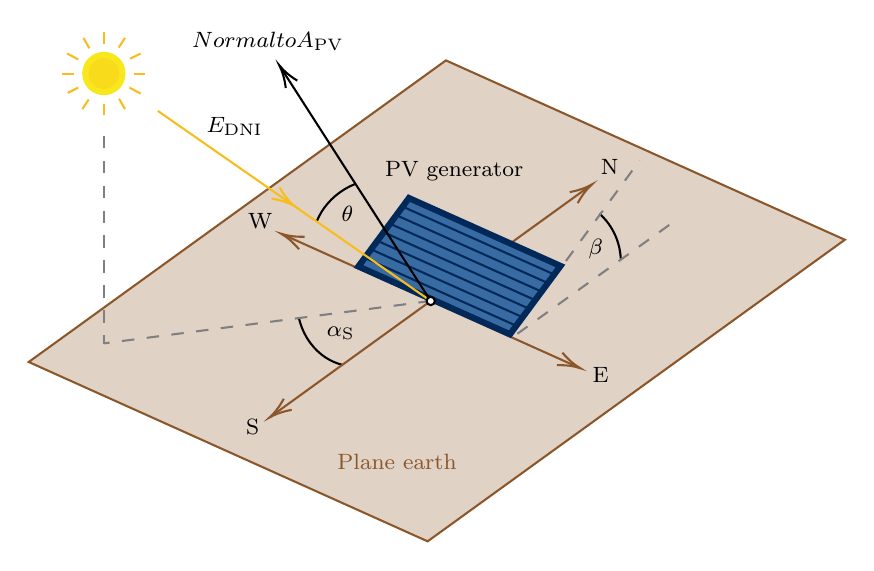
\begin{tikzpicture}[x=0.75pt,y=0.75pt,yscale=-1,xscale=1]
%uncomment if require: \path (0,455); %set diagram left start at 0, and has height of 455

%Shape: Rectangle [id:dp8474155302282593] 
\draw  [color={rgb, 255:red, 139; green, 87; blue, 42 }  ,draw opacity=1 ][fill={rgb, 255:red, 139; green, 87; blue, 42 }  ,fill opacity=0.27 ] (304.8,113.67) -- (496.99,200.08) -- (295.98,345.38) -- (103.79,258.97) -- cycle ;
%Straight Lines [id:da6680786992692076] 
\draw [color={rgb, 255:red, 139; green, 87; blue, 42 }  ,draw opacity=1 ]   (367.73,261.16) -- (227.22,197.98) ;
\draw [shift={(225.39,197.16)}, rotate = 384.21000000000004] [color={rgb, 255:red, 139; green, 87; blue, 42 }  ,draw opacity=1 ][line width=0.75]    (10.93,-3.29) .. controls (6.95,-1.4) and (3.31,-0.3) .. (0,0) .. controls (3.31,0.3) and (6.95,1.4) .. (10.93,3.29)   ;
\draw [shift={(369.56,261.98)}, rotate = 204.21] [color={rgb, 255:red, 139; green, 87; blue, 42 }  ,draw opacity=1 ][line width=0.75]    (10.93,-3.29) .. controls (6.95,-1.4) and (3.31,-0.3) .. (0,0) .. controls (3.31,0.3) and (6.95,1.4) .. (10.93,3.29)   ;
%Shape: Arc [id:dp4091032640411232] 
\draw  [draw opacity=0] (378.78,187.54) .. controls (381.04,189.51) and (383.04,191.89) .. (384.69,194.67) .. controls (387.37,199.17) and (388.78,204.17) .. (389.04,209.19) -- (360,211.71) -- cycle ; \draw   (378.78,187.54) .. controls (381.04,189.51) and (383.04,191.89) .. (384.69,194.67) .. controls (387.37,199.17) and (388.78,204.17) .. (389.04,209.19) ;
%Shape: Ellipse [id:dp7766653682919293] 
\draw  [color={rgb, 255:red, 248; green, 231; blue, 28 }  ,draw opacity=1 ][fill={rgb, 255:red, 248; green, 220; blue, 28 }  ,fill opacity=1 ][line width=2.25]  (131.06,120) .. controls (131.06,115.06) and (135.06,111.06) .. (140,111.06) .. controls (144.94,111.06) and (148.94,115.06) .. (148.94,120) .. controls (148.94,124.94) and (144.94,128.94) .. (140,128.94) .. controls (135.06,128.94) and (131.06,124.94) .. (131.06,120) -- cycle ;
%Straight Lines [id:da12322467795106329] 
\draw [color={rgb, 255:red, 248; green, 189; blue, 28 }  ,draw opacity=1 ]   (140,100) -- (140,105.56) ;
%Straight Lines [id:da4332784077616083] 
\draw [color={rgb, 255:red, 248; green, 189; blue, 28 }  ,draw opacity=1 ]   (160,120) -- (154.44,120) ;
%Straight Lines [id:da7027066659727501] 
\draw [color={rgb, 255:red, 248; green, 189; blue, 28 }  ,draw opacity=1 ]   (140,140) -- (140,134.44) ;
%Straight Lines [id:da11414191136971219] 
\draw [color={rgb, 255:red, 248; green, 189; blue, 28 }  ,draw opacity=1 ]   (125.56,120) -- (120,120) ;
%Straight Lines [id:da6688063172227983] 
\draw [color={rgb, 255:red, 248; green, 189; blue, 28 }  ,draw opacity=1 ]   (152.34,126.79) -- (157.7,129.65) ;
%Straight Lines [id:da20949775152165007] 
\draw [color={rgb, 255:red, 248; green, 189; blue, 28 }  ,draw opacity=1 ]   (122.3,110.35) -- (127.66,113.21) ;
%Straight Lines [id:da7656758253367213] 
\draw [color={rgb, 255:red, 248; green, 189; blue, 28 }  ,draw opacity=1 ]   (157.7,110.35) -- (152.65,112.85) ;
%Straight Lines [id:da9791803411373596] 
\draw [color={rgb, 255:red, 248; green, 189; blue, 28 }  ,draw opacity=1 ]   (127.66,126.79) -- (122.61,129.3) ;
%Straight Lines [id:da2234053647148624] 
\draw [color={rgb, 255:red, 248; green, 189; blue, 28 }  ,draw opacity=1 ]   (147.15,107.46) -- (150.19,102.84) ;
%Straight Lines [id:da6726326270351066] 
\draw [color={rgb, 255:red, 248; green, 189; blue, 28 }  ,draw opacity=1 ]   (129.63,137.14) -- (132.67,132.51) ;
%Straight Lines [id:da7766925486897012] 
\draw [color={rgb, 255:red, 248; green, 189; blue, 28 }  ,draw opacity=1 ]   (147.33,132.16) -- (150.19,137.16) ;
%Straight Lines [id:da3318298152117709] 
\draw [color={rgb, 255:red, 248; green, 189; blue, 28 }  ,draw opacity=1 ]   (130.17,102.84) -- (133.03,107.84) ;

%Straight Lines [id:da4654469204608218] 
\draw [color={rgb, 255:red, 128; green, 128; blue, 128 }  ,draw opacity=1 ] [dash pattern={on 4.5pt off 4.5pt}]  (140,150) -- (140,250.5) ;
%Shape: Arc [id:dp19974251160210033] 
\draw  [draw opacity=0] (255.22,260.43) .. controls (249.27,259.03) and (243.7,255.49) .. (239.53,249.88) .. controls (236.81,246.23) and (234.96,242.08) .. (233.96,237.75) -- (261.41,229.35) -- cycle ; \draw   (255.22,260.43) .. controls (249.27,259.03) and (243.7,255.49) .. (239.53,249.88) .. controls (236.81,246.23) and (234.96,242.08) .. (233.96,237.75) ;
%Straight Lines [id:da5130479264192895] 
\draw [color={rgb, 255:red, 139; green, 87; blue, 42 }  ,draw opacity=1 ]   (373.59,174.56) -- (221.36,284.59) ;
\draw [shift={(219.74,285.76)}, rotate = 324.14] [color={rgb, 255:red, 139; green, 87; blue, 42 }  ,draw opacity=1 ][line width=0.75]    (10.93,-3.29) .. controls (6.95,-1.4) and (3.31,-0.3) .. (0,0) .. controls (3.31,0.3) and (6.95,1.4) .. (10.93,3.29)   ;
\draw [shift={(375.21,173.38)}, rotate = 144.14] [color={rgb, 255:red, 139; green, 87; blue, 42 }  ,draw opacity=1 ][line width=0.75]    (10.93,-3.29) .. controls (6.95,-1.4) and (3.31,-0.3) .. (0,0) .. controls (3.31,0.3) and (6.95,1.4) .. (10.93,3.29)   ;
%Straight Lines [id:da7333561757823057] 
\draw [color={rgb, 255:red, 128; green, 128; blue, 128 }  ,draw opacity=1 ] [dash pattern={on 4.5pt off 4.5pt}]  (297.47,229.57) -- (140,250) ;
%Shape: Rectangle [id:dp9181904913709493] 
\draw  [color={rgb, 255:red, 0; green, 41; blue, 90 }  ,draw opacity=1 ][fill={rgb, 255:red, 57; green, 107; blue, 163 }  ,fill opacity=1 ][line width=2.25]  (286.99,180) -- (360,212.71) -- (335.66,245.63) -- (262.65,212.93) -- cycle ;
%Straight Lines [id:da13478383057933563] 
\draw [color={rgb, 255:red, 0; green, 41; blue, 90 }  ,draw opacity=1 ]   (283.95,184.12) -- (356.96,216.82) ;
%Straight Lines [id:da5884374823291068] 
\draw [color={rgb, 255:red, 0; green, 41; blue, 90 }  ,draw opacity=1 ]   (265.69,208.81) -- (338.7,241.52) ;
%Straight Lines [id:da02285619917411874] 
\draw [color={rgb, 255:red, 0; green, 41; blue, 90 }  ,draw opacity=1 ]   (268.74,204.7) -- (341.75,237.4) ;
%Straight Lines [id:da23820193833800274] 
\draw [color={rgb, 255:red, 0; green, 41; blue, 90 }  ,draw opacity=1 ]   (271.78,200.58) -- (344.79,233.28) ;
%Straight Lines [id:da14178706586084355] 
\draw [color={rgb, 255:red, 0; green, 41; blue, 90 }  ,draw opacity=1 ]   (280.9,188.23) -- (353.91,220.94) ;
%Straight Lines [id:da14421525428340431] 
\draw [color={rgb, 255:red, 0; green, 41; blue, 90 }  ,draw opacity=1 ]   (274.82,196.46) -- (347.83,229.17) ;
%Straight Lines [id:da3643942316695261] 
\draw [color={rgb, 255:red, 0; green, 41; blue, 90 }  ,draw opacity=1 ]   (277.86,192.35) -- (350.87,225.05) ;
%Shape: Arc [id:dp7190646059564607] 
\draw  [draw opacity=0] (242.59,191.14) .. controls (245.03,185.16) and (249.56,179.68) .. (255.82,175.84) .. controls (257.47,174.83) and (259.17,173.97) .. (260.9,173.27) -- (269.51,198.17) -- cycle ; \draw   (242.59,191.14) .. controls (245.03,185.16) and (249.56,179.68) .. (255.82,175.84) .. controls (257.47,174.83) and (259.17,173.97) .. (260.9,173.27) ;
%Straight Lines [id:da4133530859205612] 
\draw [color={rgb, 255:red, 248; green, 189; blue, 28 }  ,draw opacity=1 ][line width=0.75]    (166,138) -- (230.1,182.64) ;
\draw [shift={(231.74,183.79)}, rotate = 214.86] [color={rgb, 255:red, 248; green, 189; blue, 28 }  ,draw opacity=1 ][line width=0.75]    (10.93,-3.29) .. controls (6.95,-1.4) and (3.31,-0.3) .. (0,0) .. controls (3.31,0.3) and (6.95,1.4) .. (10.93,3.29)   ;
%Straight Lines [id:da8270043512595768] 
\draw [color={rgb, 255:red, 248; green, 189; blue, 28 }  ,draw opacity=1 ][line width=0.75]    (231.74,183.79) -- (297.47,229.57) ;
%Straight Lines [id:da7037472432355609] 
\draw [color={rgb, 255:red, 0; green, 0; blue, 0 }  ,draw opacity=1 ]   (297.47,229.57) -- (225.58,117.68) ;
\draw [shift={(224.5,116)}, rotate = 417.28] [color={rgb, 255:red, 0; green, 0; blue, 0 }  ,draw opacity=1 ][line width=0.75]    (10.93,-3.29) .. controls (6.95,-1.4) and (3.31,-0.3) .. (0,0) .. controls (3.31,0.3) and (6.95,1.4) .. (10.93,3.29)   ;
%Straight Lines [id:da7634900279620906] 
\draw [color={rgb, 255:red, 128; green, 128; blue, 128 }  ,draw opacity=1 ] [dash pattern={on 4.5pt off 4.5pt}]  (412.4,192.95) -- (334.66,248.63) ;
%Straight Lines [id:da3198763131888107] 
\draw [color={rgb, 255:red, 128; green, 128; blue, 128 }  ,draw opacity=1 ] [dash pattern={on 4.5pt off 4.5pt}]  (362.64,210.28) -- (398.15,161.88) ;
%Shape: Circle [id:dp009625788709507033] 
\draw  [fill={rgb, 255:red, 255; green, 255; blue, 255 }  ,fill opacity=1 ] (295.47,229.57) .. controls (295.47,228.47) and (296.37,227.57) .. (297.47,227.57) .. controls (298.58,227.57) and (299.47,228.47) .. (299.47,229.57) .. controls (299.47,230.68) and (298.58,231.57) .. (297.47,231.57) .. controls (296.37,231.57) and (295.47,230.68) .. (295.47,229.57) -- cycle ;

% Text Node
\draw (372,198.4) node [anchor=north west][inner sep=0.75pt]  [font=\footnotesize]  {$\beta $};
% Text Node
\draw (378,160) node [anchor=north west][inner sep=0.75pt]  [font=\footnotesize] [align=left] {N};
% Text Node
\draw (207,285) node [anchor=north west][inner sep=0.75pt]  [font=\footnotesize] [align=left] {S};
% Text Node
\draw (374,260) node [anchor=north west][inner sep=0.75pt]  [font=\footnotesize] [align=left] {E};
% Text Node
\draw (208,186) node [anchor=north west][inner sep=0.75pt]  [font=\footnotesize] [align=left] {W};
% Text Node
\draw (274,161) node [anchor=north west][inner sep=0.75pt]  [font=\footnotesize] [align=left] {PV generator};
% Text Node
\draw (246,240.4) node [anchor=north west][inner sep=0.75pt]  [font=\footnotesize]  {$\alpha _{\mathrm{S}}$};
% Text Node
\draw (253,182.4) node [anchor=north west][inner sep=0.75pt]  [font=\footnotesize]  {$\theta $};
% Text Node
\draw (251,302) node [anchor=north west][inner sep=0.75pt]  [font=\footnotesize,color={rgb, 255:red, 139; green, 87; blue, 42 }  ,opacity=1 ] [align=left] {Plane earth};
% Text Node
\draw (188,139.4) node [anchor=north west][inner sep=0.75pt]  [font=\footnotesize]  {$E_{\mathrm{DNI}}$};
% Text Node
\draw (181,98.4) node [anchor=north west][inner sep=0.75pt]  [font=\footnotesize]  {$\text{Normal to } A_{\mathrm{PV}}$};


\end{tikzpicture}

	\caption{Illustration of the incidence angle $\theta$ of the solar rays with respect to the normal to $A_\mathrm{PV}$. (Recreated from: \cite{Landis:1995})}
	\label{fig:tikz_angle_theta}
\end{figure}
The angle of incidence $\theta$ has a range of $\left[0^\circ \text{, } 90^\circ\right]$ and $\alpha_\mathrm{S}(t_\mathrm{S} = 12\mathrm{h})$ represents the orientation of the normal to $A_\mathrm{PV}$. For completenes it must be mentioned that equation (\ref{eq:sin_gamma_s}) can be derived from equation (\ref{eq:cos_theta}) with $\beta = 0^\circ$, and that in the case $\gamma_{\mathrm{S}} + \beta = 90^\circ$, the Sun's rays are perpendicular to the PV generator's energy-converting area $A_{\mathrm{PV}}$ which results in $E_{\mathrm{DGI}} = E_{\mathrm{DNI}}$ \cite{Landis:1995, Bertol:2011, Mertens:2015, Wagner:2018}.

To determine the second component from equation (\ref{eq:e_gen}) the sky is assumed to be isotropic. This means that the DIFH is evenly distributed in the entire celestial hemisphere above the PV generator. The more the PV generator is inclined the smaller the proportion of DIFG in equation (\ref{eq:e_difg}) becomes (compare to figure \ref{fig:tikz_three_component_model}) \cite{Landis:1995, Mertens:2015}. 
	\begin{equation} \label{eq:e_difg}
	\centering
		E_{\mathrm{DIFG}} = E_{\mathrm{DIFH}} \, \frac{1 + \cos \beta }{2}
	\end{equation} 
In the book \cite{Mertens:2015} it is expressly pointed out that the isotropic approach used in equation (\ref{eq:e_difg}) is only a rough approximation. This is because the sky is brighter towards the Sun than towards the horizon.\footnote{More precise equations would be difficult to derive, which would go beyond the scope of this thesis.} 

When examining the last component from equation (\ref{eq:e_gen}) it has to be taken into account that different surfaces -- on which a PV generator is placed -- reflect solar rays differently. In equation (\ref{eq:e_rgi}) this is accomplished with the factor $\mathrm{ALB}$ -- also known as the reflectivity. Similar to equation (\ref{eq:e_difg}) an isotropic approach is used \cite{Landis:1995, Dobos:2011, Mertens:2015, Bralower:2018}. 
	\begin{equation} \label{eq:e_rgi}
	\centering
		E_{\mathrm{RGI}} = E_{\mathrm{GHI}} \, \frac{1 - \cos \beta }{2} \cdot \mathrm{ALB}
	\end{equation}
Approximate albedo values for various surfaces are listed in table \ref{tab:table_albedo}. The larger the value the more solar rays are reflected. A blackbody for example has an albedo value of 0 while an absolute white surface has an albedo value of 1. The Earth has an average albedo of 0,31 \cite{Bennett:2010, Dobos:2011, Bralower:2018}.
\begin{table}[h!]
	\centering
	\footnotesize
\begin{tabular}{|l|c|l|c|}
	\hline
	\textbf{Surface} & \textbf{Albedo} & \textbf{Surface} & \textbf{Albedo} \\
	\hline
	Forest & 0,05 -- 0,18 & Sand & 0,20 -- 0,40 \\
	Water & 0,06 -- 0,10 & Grass (July, August) & 0,25 \\
	Rain forest & 0,07 -- 0,15 & Dry sandy soil & 0,25 -- 0,45 \\
	Coniferous forest & 0,09 -- 0,15 & Uncultivated field & 0,26 \\
	Dark-colored soil surfaces & 0,10 -- 0,20 & New concrete & 0,30 \\
	Heathland & 0,10 -- 0,25 & Granite & 0,30 -- 0,35 \\
	Asphalt & 0,15 & Glacial ice & 0,30 -- 0,40 \\
	Deciduous forest & 0,15 -- 0,18 & Light-colored soil surfaces & 0,40 -- 0,50 \\
	Dry clay soil & 0,15 -- 0,35 & Old snow & 0,45 -- 0,70 \\
	Lawn & 0,18 -- 0,23 & Dry salt cover & 0,50 \\
	Weathered concrete & 0,20 & Fresh snow & 0,80 -- 0,90 \\
	\hline
\end{tabular}
	\caption{Albedo values (refelctivity) for different surfaces \cite{Dobos:2011, Bertol:2011, Mertens:2015, Bralower:2018}.}
	\label{tab:table_albedo}
\end{table}

If the three derived components $E_{\mathrm{DGI}}$, $E_{\mathrm{DIFG}}$ and $E_{\mathrm{RGI}}$ are now inserted into equation (\ref{eq:e_gen}) while considering the equations (\ref{eq:e_ghi}) and (\ref{eq:e_dni}), the total irradiance $E_{\mathrm{G}}$ received by an inclined PV generator, depending on $E_{\mathrm{GHI}}$, $E_{\mathrm{DNI}}$, $\gamma_{\mathrm{S}}$, $\beta$ and $\mathrm{ALB}$, can be obtained:
	\begin{equation} \label{eq:e_gen_ghi_dni}
	\centering
		\begin{split}
		E_{\mathrm{G}} = E_{\mathrm{DNI}} \, \cos \theta + \left(E_{\mathrm{GHI}} - E_{\mathrm{DNI}} \, \sin \gamma_{\mathrm{S}}\right) \frac{1 + \cos \beta }{2} \\ 
		+ E_{\mathrm{GHI}} \, \frac{1 - \cos \beta }{2} \cdot \mathrm{ALB} \text{.}
		\end{split}
	\end{equation}
Regarding this equation it must be noted that the angles $\gamma_{\mathrm{S}}$ and $\theta$ are time dependent and therefore $E_{\mathrm{G}}$ as well. $E_{\mathrm{GHI}}$ and $E_{\mathrm{DNI}}$ on the other hand are average values -- if taken from solar resource maps -- and can therefore be treated as constants. The angle of inclination $\beta$ as well as the albedo value $\mathrm{ALB}$ are also treated as constants. Once the PV generator is installed its inclination angle $\beta$ will not change for the entire duration of the mission. This has the consequence that the PV generator's inclined energy-converting area $A_{\mathrm{PV}}$ is only perpendicular for one pair of $\gamma_{\mathrm{S}}$ and $\alpha_{\mathrm{S}}$ at a given time of the day. Even though $\mathrm{ALB}$ is treated as a constant, there are situations in which the albedo value of a surface can change over the course of a few hours. For instance, if the PV generator is installed on a freshly snowed uncultivated field and the snow melts away. In this case $\mathrm{ALB}$ would change from 0,80 to 0,26. Such situations must be considered while simulating the PV generator's daily energy yield. This can be accomplished by considering the lowest possible albedo value for a given region \cite{Appelbaum:1992, Landis:1995, Mertens:2015}.

As described by \cite{Mertens:2015, Wagner:2018}, the radiation flux $\Phi_{\mathrm{G}}$ onto the PV generator's energy-converting area $A_{\mathrm{PV}}$ -- to be more precise the sum of the energy-converting area of the PV cells -- can be calculated as follows:
	\begin{equation} \label{eq:radiation_flux}
	\centering
		\Phi_{\mathrm{G}} = A_{\mathrm{PV}} \, E_{\mathrm{G}}\text{.} 
	\end{equation}

How to determine the optimal angle of inclination $\beta$ for a PV generator will be discussed in the next subsection.
